\documentclass{article}
% --- watermark (auto-inserted) ---
\usepackage{xcolor}
\usepackage{xfp}% \fpeval; in the kernel since 2022, harmless on older LaTeX
\usepackage{draftwatermark}
\newlength{\watermarkTextWidth}
\AddToHook{begindocument/end}{%
  \SetWatermarkText{\normalfont Generated by The Agentic Scientist}%
  \SetWatermarkFontSize{10pt}%
  \SetWatermarkLightness{0.85}%
  \settowidth{\watermarkTextWidth}{\normalfont\fontsize{10pt}{12pt}\selectfont Generated by The Agentic Scientist}%
  \edef\watermarkScale{\fpeval{0.8 * sqrt(\paperwidth**2 + \paperheight**2) / \watermarkTextWidth}}%
  \edef\watermarkAngle{\fpeval{atand(\paperheight/\paperwidth)}}%
  \SetWatermarkScale{\watermarkScale}%
  \SetWatermarkAngle{\watermarkAngle}%
}
% --- end watermark ---

\usepackage{paper,times}
\usepackage[T1]{fontenc}
\usepackage[utf8]{inputenc}
\usepackage{amsmath,amssymb,booktabs,graphicx,subcaption}
\usepackage{hyperref,url}
\title{Score-Targeted Item Selection for LLM Benchmark Prediction:\\Accuracy and Evaluation Limits}
\author{}
\newcommand{\clip}{\operatorname{clip}_{[0,1]}}
\newcommand{\sigmoid}{\operatorname{sigmoid}}
\begin{document}
\maketitle

\begin{abstract}
Predicting a language model's benchmark score from a few responses can reduce evaluation cost, but prediction accuracy and evaluation completeness are different requirements. We study a source-only estimator that selects items by their conditional covariance with the full score and combines ridge prediction with an optional Rasch-residual profile mixture. A frozen evaluation covers ten fixed benchmark cases, three grouped model splits, and budgets of 8, 16, and 32 items. On common available support, the estimator's mean absolute error decreases from 0.0439 to 0.0278 across these budgets; its Spearman correlation increases from 0.7787 to 0.8858. These are conditional descriptions, not qualified overall results. The evaluation completed but failed qualification: primary and reference predictions are missing for two Commonsense splits, and matched structural checks fail. The reported aggregate MAE of 0.0880 includes missing-output penalties. We separate measured prediction errors, scoring defaults, and unresolved diagnostics, establishing an evidence-bounded assessment rather than an overall selection-advantage claim.
\end{abstract}
% @evidence[[paper_data.json#/final_evaluation]]
% @evidence[[derived_results.json#/budget_mae]]
% @evidence[[derived_results.json#/budget_spearman]]

\section{Introduction}
Full-benchmark evaluation repeatedly measures the same item universe across language models, checkpoints, or inference settings. Historical item-level responses may therefore contain useful information about which questions distinguish model behavior. The practical question is whether a new model can answer a small, fixed subset while a source-trained estimator reconstructs its full score and preserves model rankings. This setting differs from accelerating generation: the savings come from querying fewer items, not from changing the evaluated language model.

Existing benchmark-compression methods exploit response similarity, latent ability, or predictive dependencies \citep{Vivek2024,Polo2024,Kipnis2025,Pacchiardi2024,Li2025}. A complementary design objective is to select questions directly for the scalar score of interest. An item can distinguish source response patterns without being especially informative about their average. Conversely, correlated items can remain useful if their residual variation predicts that average. This motivates conditioning on already selected items and greedily targeting the remaining covariance with the full source score.

We study this design together with a source-trained reconstruction family. A linear ridge predictor provides a simple fallback; a group-balanced mixture of Rasch-shrunk source profiles offers nonlinear response-pattern matching. Both use the same nested item prefixes, and their combination is selected using source-group holdouts. The scientific hypothesis is that source response structure can improve score reconstruction at a fixed query budget. The available evaluation does not isolate a benefit from the profile component, nor does it establish a generally advantageous selector.

The decisive evidence boundary is evaluation integrity. The frozen assessment completed but did not qualify. Missing primary predictions coincide with missing reference predictions in part of the Commonsense evidence; matched structural checks also fail there. The retained predictions can describe accuracy on available pairs, but cannot supply the missing outcomes or restore qualification. Treating penalty-scored aggregate errors as ordinary prediction errors would obscure this distinction.
% @evidence[[paper_data.json#/final_evaluation/outcome]]
% @evidence[[paper_data.json#/final_evaluation/evaluation_evidence/episodes]]

Our contributions are consequently bounded: a precise description of a score-targeted, source-only reconstruction method; a common-support comparison across fixed benchmarks and item budgets; and an explicit account of how incomplete records restrict the interpretation of those comparisons. We report the unsuccessful qualification alongside the conditional results rather than selecting whichever summary gives the most favorable ordering. The resulting study addresses what these measurements establish, and what remains unmeasured.

\begin{figure}[t]
\centering

\includegraphics[width=\linewidth]{figures/method_and_evidence_overview.png}
\caption{Source-only item design and score reconstruction, with an explicit evidence boundary. Source responses determine a fixed nested item order, ridge fitting, and an optional residual-profile mixture. Target responses update prediction only. Measured prediction error is distinguished from missing records and failed checks; the latter cannot be repaired by conditioning on available predictions.}
\label{fig:overview}
\end{figure}

\section{Related Work}
\paragraph{Few-item language-model evaluation.}
Anchor Points selects a small set of representative examples from cross-model response structure \citep{Vivek2024}. tinyBenchmarks studies efficient score estimation with curated subsets, and metabench uses latent abilities to compress reasoning and knowledge evaluation \citep{Polo2024,Kipnis2025}. Reference-instance assessors predict model performance on other instances \citep{Pacchiardi2024}; learned evaluation-acquisition policies model dependencies between test outcomes \citep{Li2025}. Our fixed source-only order is not target-adaptive acquisition. The local anchor and IRT references below are explicitly defined implementations, not certified reproductions of these published systems.

\paragraph{Design and reconstruction.}
Choosing observations for a scalar target relates to optimal allocation in regression \citep{Elfving1952}, whereas information criteria for a whole parameter vector address a different objective \citep{Kiefer1960}. Our empirical covariance rule is a regularized linear-prediction heuristic, not an optimal-design theorem for shifted binary responses. Ridge regression supplies a stabilized linear estimator \citep{Hoerl1970}; standard statistical-learning and probabilistic-modeling texts provide broader background \citep{Hastie2009,Bishop2006}. The profile model is a finite mixture, but it does not fit mixture weights by expectation maximization \citep{Dempster1977}. Likewise, its fixed-ability difficulty fitting should not be confused with conditional maximum-likelihood estimation \citep{Andersen1970}.

\paragraph{Assessment under dependence and missingness.}
Cross-validation distinguishes choosing a predictor from assessing it \citep{Stone1974,Arlot2010}; evaluating a configuration on the same validation evidence used to tune it can be optimistic \citep{Varma2006}. Grouped validation addresses dependence, but the blocking scheme determines which extrapolation question is tested \citep{Roberts2017}. Domain-shift theory further motivates caution about transferring source accuracy to new response distributions \citep{BenDavid2010}. Missing-data inference requires assumptions about the missingness process \citep{Rubin1976,Little2019}; we make no such assumptions here. HELM motivates multi-metric evaluation \citep{Liang2023}, and distinct benchmark constructions, such as MMLU-Pro, should not be conflated with the fixed MMLU case studied here \citep{Wang2024}. These distinctions motivate reporting error, ranking, and evidence availability separately.

\section{Method}
\subsection{Problem Setup and Design Rationale}
Let $X\in\{0,1\}^{S\times N}$ contain complete item responses of source models, and let $y\in\{0,1\}^{N}$ denote a target model's responses. Its reference score is $s(y)=N^{-1}\sum_{j=1}^{N}y_j$. Only $y_Q$ is observable to the estimator, for a subset $Q$ of size $b\ll N$. Source rows have supplied group labels $g(i)$; target identities, target groups, and full target scores are unavailable during fitting and prediction. The goal is a bounded estimate $\hat s_b(y_Q)$ with small absolute and squared score error and accurate target-model ordering.

The studied budgets are $b\in\{8,16,32\}$. A single source-only order gives nested prefixes $Q_b$, with no repeated items. This is not a claim that these budgets suffice for every benchmark. The rationale is to combine task-directed acquisition with conservative reconstruction: selection targets the full-score functional, while a tuned linear fallback limits reliance on an overly specific source-profile model. Equal total source-group mass reduces the influence of densely represented groups in selection and profile priors, without asserting that groups perfectly recover training ancestry.
% @evidence[[paper_data.json#/final_evaluation/evaluation_evidence/episodes/0/solution/budgets]]
% @evidence[[source_evidence/selected_method.py#L1-L28]]

\subsection{Score-Targeted Fixed Prefixes}
For $G$ source groups with sizes $n_g$, define $w_i=(G n_{g(i)})^{-1}$, source item means $\mu_j=\sum_i w_iX_{ij}$, and full source scores $t_i=N^{-1}\sum_jX_{ij}$. With $\bar t=\sum_iw_it_i$, form
\begin{equation}
 Z_{ij}=\sqrt{w_i}(X_{ij}-\mu_j),\qquad
 u_i=\sqrt{w_i}(t_i-\bar t),\quad
 C=Z^\top Z+D,\quad c=Z^\top u,
\end{equation}
where $D_{jj}=0.1\max\{\mu_j(1-\mu_j),0.05\}$. For the selected prefix $Q$, residual covariance and variance are
\begin{equation}
 c_{j\mid Q}=c_j-C_{jQ}C_{QQ}^{-1}c_Q,\qquad
 v_{j\mid Q}=C_{jj}-C_{jQ}C_{QQ}^{-1}C_{Qj}.
\end{equation}
The next item maximizes $c_{j\mid Q}^{\,2}/\max(v_{j\mid Q},10^{-12})$ among unselected items. This is the reduction in residual variance for a linear scalar-score predictor under the empirical covariance model. It is neither an information guarantee for the true target distribution nor a causal statement about particular questions.
% @evidence[[source_evidence/selected_method.py#L57-L91]]

The implementation updates residual quantities through a low-rank pivoted factorization instead of materializing the dense item covariance. Selection is rebuilt using only training groups inside every source-validation fold. The final fit repeats it on all supplied source rows. Crucially, observing target answers never changes the item order or its hyperparameters.

\subsection{Linear and Residual-Profile Reconstruction}
The linear branch regresses source full scores on the selected binary responses. Centering features at their unweighted source mean $\bar x_Q$ and scores at $\bar t_{\rm row}$ gives
\begin{equation}
 \beta_b=(X_{Q,c}^{\top}X_{Q,c}+\lambda I)^{-1}X_{Q,c}^{\top}(t-\bar t_{\rm row}),\qquad
 \hat s^{\rm lin}_b=\clip\!\left[\bar t_{\rm row}+\gamma(y_Q-\bar x_Q)^\top\beta_b\right].
\end{equation}
The ridge fit itself is row-unweighted; group balancing is used for selecting configurations, not silently substituted into this regression. Per-budget $\lambda\in\{0.1,1,10\}$ and $\gamma\in\{0,0.5,1\}$ minimize source-held-out group-weighted squared error.
% @evidence[[source_evidence/selected_method.py#L94-L100]]
% @evidence[[source_evidence/selected_method.py#L200-L270]]

% @evidence[[reference_consultation.md#targeted-irt-foundations]]
The nonlinear branch retains source response profiles while smoothing them with a Rasch response model, a logistic ability--difficulty family \citep[Chap.~2]{Baker2001}. Our custom fit fixes source abilities at $\theta_i=\operatorname{logit}[(\sum_jX_{ij}+0.5)/(N+1)]$. Item difficulties $d_j$ are fitted by group-weighted Bernoulli likelihood with a quadratic penalty. Write $r_{ij}=\sigmoid(\theta_i-d_j)$ and
\begin{equation}
 p_{ij}=\operatorname{clip}_{[\epsilon,1-\epsilon]}
       [(1-\rho)r_{ij}+\rho X_{ij}],\qquad
 p_{i\ell j}=\sigmoid[\operatorname{logit}(p_{ij})+a_\ell].
\end{equation}
The offsets are $a_\ell=h(-2,-1,0,1,2)_\ell$ with prior proportions $(1,4,6,4,1)/16$. Each source group's total prior mass is equal; within a group it is divided equally across source rows. Thus this is a mixture of source-derived response profiles and ability offsets, not a new language-model architecture.
% @evidence[[source_evidence/selected_method.py#L103-L141]]

For observed responses, a particle $k=(i,\ell)$ receives posterior mass
\begin{equation}
 \omega_k(y_Q)\ \propto\ \pi_k\prod_{j\in Q}p_{kj}^{y_j}(1-p_{kj})^{1-y_j},\qquad
 \hat s^{\rm prof}_b=\frac{\sum_{j\in Q}y_j+\sum_k\omega_k\sum_{j\notin Q}p_{kj}}{N}.
\label{eq:profile}
\end{equation}
The observed contribution is exact; only unqueried responses are reconstructed. Log-sum-exp normalization stabilizes the calculation. Every request uses the original prior and the complete current prefix, so cumulative responses are not counted twice. This model-based posterior is not an empirically calibrated uncertainty interval.
% @evidence[[source_evidence/selected_method.py#L158-L191]]

The output is $(1-\alpha)\hat s^{\rm lin}_b+\alpha\hat s^{\rm prof}_b$. Source tuning considers $\rho\in\{0,0.5,0.75\}$, $h\in\{0,0.5\}$, and $\alpha\in\{0,0.5,1\}$, using at most three group-disjoint folds. It selects one profile/blend configuration across budgets by equal-group held-out MAE. Ties favor smaller blend weight, offset scale, then residual weight. A zero blend is an explicit linear fallback. The final evidence does not record which blend was used in each fit, so it cannot demonstrate a nonzero profile contribution.
% @evidence[[source_evidence/selected_method.py#L194-L287]]

\subsection{What a Fixed Prefix Can Identify}
The reconstruction problem has an information constraint independent of the chosen statistical model. If two target models have identical queried responses, the interface supplies no information that could distinguish them, so the estimator returns the same value. In particular, neither target identities nor target group memberships are additional inputs to prediction. The source-trained mappings and particle priors are also identical for these rows. A fixed prefix therefore cannot distinguish targets that agree on observed items but differ elsewhere. We do not measure the prevalence of such pairs in the final evidence: the available score records do not supply the queried response patterns needed for that analysis. This source-inspectable property explains why score covariance is a design rationale rather than a target-level guarantee. Undocumented target response patterns may remain indistinguishable even when source-held-out prediction looks accurate.
% @evidence[[source_evidence/selected_method.py#L336-L365]]

The two reconstruction branches make different assumptions about this unresolved information. The linear branch extends source score relationships through a regularized affine map. The profile branch assigns probability to source-shaped patterns with ability offsets, then averages their unobserved totals. The convex fallback prevents source tuning from requiring the profile branch, but does not protect against shifts absent from every validation group. Neither branch acquires new target information beyond the prescribed prefix. Increasing the number of particles or retuning the blend therefore cannot by itself resolve identical-prefix ambiguity. Conversely, replacing the item order may change which targets become indistinguishable, but its effect cannot be assigned to acquisition alone when the reconstruction is also refitted. This motivates keeping the procedure-level and matched-order comparisons separate in the results.

\section{Evaluation Protocol and Evidence Availability}
\subsection{Fixed Benchmarks and Grouped Model Holdouts}
% @evidence[[reference_consultation.md#targeted-collection-context]]
The final assessment contains four Open LLM Leaderboard-derived cases (BBH, GPQA, MuSR, and OpenLLM Math) and six HELM-derived cases (Commonsense, GSM, LegalBench, MATH, MedQA, and MMLU). The upstream collections are documented by \citet{OpenLLMLeaderboard} and \citet{Liang2023}, respectively; our case identities and filtering come from the supplied data manifest. We retain these staged case names rather than asserting identity with every similarly named public benchmark. Each case uses a fixed binary item universe. The question is prediction for held-out models on that universe, not generalization to newly sampled questions or unseen benchmark distributions.
% @evidence[[paper_data.json#/final_evaluation/evaluation_evidence/episodes/0/solution/cases]]
% @evidence[[source_evidence/final_data_manifest.json]]

Seeds 5003, 7001, and 9001 define model-group splits. The evaluator orders groups by a seed-dependent hash, assigns approximately 70\% of groups to the source side, and withholds the rest as targets. Group construction uses available provenance and conservative family/provider information. It is a metadata heuristic, not a proof of disjoint pretraining or complete ancestry separation. The estimator sees only opaque source-group labels. Source tuning is internal to a fit; final targets are not used to select its settings. Repeated seeds reuse model populations and are not independent populations.
% @evidence[[paper_data.json#/final_evaluation/evaluation_evidence/episodes]]
% @evidence[[source_evidence/evaluate_final.py#L685-L708]]
% @evidence[[source_evidence/final_data_manifest.json#/split_rule]]

\subsection{Comparators and Control Semantics}
The \emph{fitted uniform-selection control} replaces the score-targeted order with a seeded uniform nested order, rebuilding selection and tuning in each fold. It keeps the reconstruction family, not necessarily the fitted predictor: hyperparameters can change. The \emph{selected-item mean} retains the primary order and returns the raw observed mean, removing reconstruction as a whole rather than an affine calibration layer. The \emph{uniform sample mean} averages responses on the same seeded uniform order used by the fitted uniform control, permitting a second matched-order reconstruction comparison.
% @evidence[[source_evidence/selected_method.py#L57-L62]]
% @evidence[[source_evidence/selected_method.py#L327-L365]]
% @evidence[[source_evidence/evaluate_final.py#L774-L840]]

The anchor reference clusters centered, normalized item response vectors and estimates scores from representatives weighted by assigned cluster sizes. The IRT reference fits a penalized two-parameter logistic response model, chooses items by fitted information near zero ability, and infers target ability from queried responses; the response family and item-information definition follow standard IRT terminology \citep[Chaps.~2,6]{Baker2001}. These references use the same query budgets, but they are local comparators, not official reproductions of Anchor Points or tinyBenchmarks. A source-mean reference predicts the average source score without target responses. Extended fitting details are in the supplement.
% @evidence[[source_evidence/evaluate_final.py#L711-L771]]

\subsection{Three Distinct Reporting Objects}
We distinguish (i) the evaluator's reported aggregate, (ii) prediction errors computed on common available records, and (iii) qualification and structural diagnostics. In the reported aggregate, the two data sources receive equal mass, cases are equally weighted within source, and seeds and budgets are equally weighted. Missing predictions receive worst-case defaults: MAE and RMSE are set to one, and rank correlations to minus one. Absent baseline records similarly receive MAE one. These defaults are operational penalties, not measured model predictions.
% @evidence[[source_evidence/evaluate_final.py#L870-L873]]
% @evidence[[source_evidence/evaluate_final.py#L1005-L1042]]

For conditional comparisons, all displayed methods must have predictions for a case--seed pair. We average budgets and targets within that pair and show its seed-level values. Pooled conditional summaries retain equal data-source and case weights, but normalize seed weights over available seeds \emph{within each case}. The same availability intersection is used for error and ranking in the budget view. Commonsense therefore contributes only its available split, rather than being silently omitted or assigned a synthetic loss. This changes the estimand; it does not estimate missing performance. We show descriptive seed dispersion, not confidence bars. Spearman and Kendall correlations describe ordering \citep{Spearman1904,Kendall1938}; neither establishes score calibration.
% @evidence[[derived_results.json#/common_support]]

\section{Results}
\subsection{Completed Evaluation, Failed Qualification}
The final evaluation completed and failed qualification. Table~\ref{tab:aggregate} preserves its scored summaries. Primary MAE is 0.0880 and RMSE is 0.0979; reported Spearman and Kendall correlations are 0.7329 and 0.5943. These summaries include defaults for missing primary records. Their ordering against the fitted uniform-selection MAE of 0.0449 cannot be interpreted as a measured overall selection disadvantage.
% @evidence[[paper_data.json#/final_evaluation/metrics]]
% @evidence[[paper_data.json#/final_evaluation/outcome]]

\begin{table}[t]
\centering
\caption{Reported final aggregates, \emph{including evaluator defaults}. Errors are score fractions. Missing primary and baseline records receive error one; fitted controls have different availability. These columns are not a measured-only superiority ranking.}
\label{tab:aggregate}
\begin{tabular}{lr@{\qquad}lr}
\toprule
Prediction rule & MAE & Primary diagnostic & Value\\
\midrule
Score-targeted reconstruction & 0.0880 & RMSE & 0.0979\\
Uniform selection + fitting & 0.0449 & Spearman & 0.7329\\
Selected-item mean & 0.1084 & Kendall $\tau_b$ & 0.5943\\
Uniform sample mean & 0.1336 & Structural-control failure summary & 0.0417\\
IRT reference & 0.1187 & Missing-evaluation fraction & 0.0110\\
Anchor reference & 0.2205 & Checked replay discrepancy & 0.0000\\
Source-mean reference & 0.1644 & Qualification & Failed\\
\bottomrule
\end{tabular}
\end{table}
% @evidence[[paper_data.json#/final_evaluation/metrics]]

The failure evidence is localized but consequential (Table~\ref{tab:audit}). Primary predictions and all reference predictions are absent for Commonsense at seeds 5003 and 9001. Constant, copied, permuted, and selected-item-mean conditions have recorded predictions there but fail structural checks. The fitted uniform control is available there. The retained record does not identify the underlying exception or root defect, so missing outputs should not be described as an accuracy failure, and the failed checks should not be attributed to a particular implementation error without additional evidence.
% @evidence[[paper_data.json#/final_evaluation/evaluation_evidence/episodes]]

\begin{table}[t]
\centering
\caption{Availability and integrity audit of the final evidence. The two affected Commonsense splits are not counted as measured prediction losses in our conditional figures.}
\label{tab:audit}
\begin{tabular}{p{.30\linewidth}p{.60\linewidth}}
\toprule
Evidence & Recorded finding\\
\midrule
Commonsense, seeds 5003/9001 & Primary and reference predictions absent; matched constant, copy, permutation, and selected-mean structural checks fail.\\
Common comparison support & 28 of 30 case--seed pairs; Commonsense uses seed 7001 only.\\
Paired primary--anchor contrast & $-0.0769$ with stored endpoints $[-1,1]$; endpoints are fallback values, not an informative interval.\\
Reset replay & Maximum absolute discrepancy $0$ for the checked replay; not a certificate for other conditions.\\
\bottomrule
\end{tabular}
\end{table}
% @evidence[[derived_results.json#/common_support]]
% @evidence[[paper_data.json#/final_evaluation/metrics/delta_anchor_mae]]
% @evidence[[source_evidence/evaluate_final.py#L1040-L1074]]

The paired primary--anchor contrast has a separate missing-record convention. It is not obtained by subtracting the separately penalized aggregate MAEs. Its stored interval endpoints remain the evaluator's initialized fallback because complete pairing is unavailable. We therefore report no significance claim. Bootstrap methodology \citep{Efron1979} does not turn unexecuted or unsupported resampling into an uncertainty estimate.

\subsection{Conditional Comparison Across Fixed Cases}
Figure~\ref{fig:cases} compares only common available predictions. The primary estimator has lower descriptive MAE than the fitted uniform control in nine cases; MedQA is the exception (0.0574 versus 0.0530). This count includes Commonsense with only one supported seed. BBH gives 0.0308 versus 0.0570, while the corresponding values on MATH are 0.0603 and 0.0624. Thus the observed differences vary substantially across cases. The anchor reference's especially large MuSR error also illustrates why a single pooled comparator should not substitute for the case-level view.
% @evidence[[derived_results.json#/case_mae]]

\begin{figure}[t]
\centering
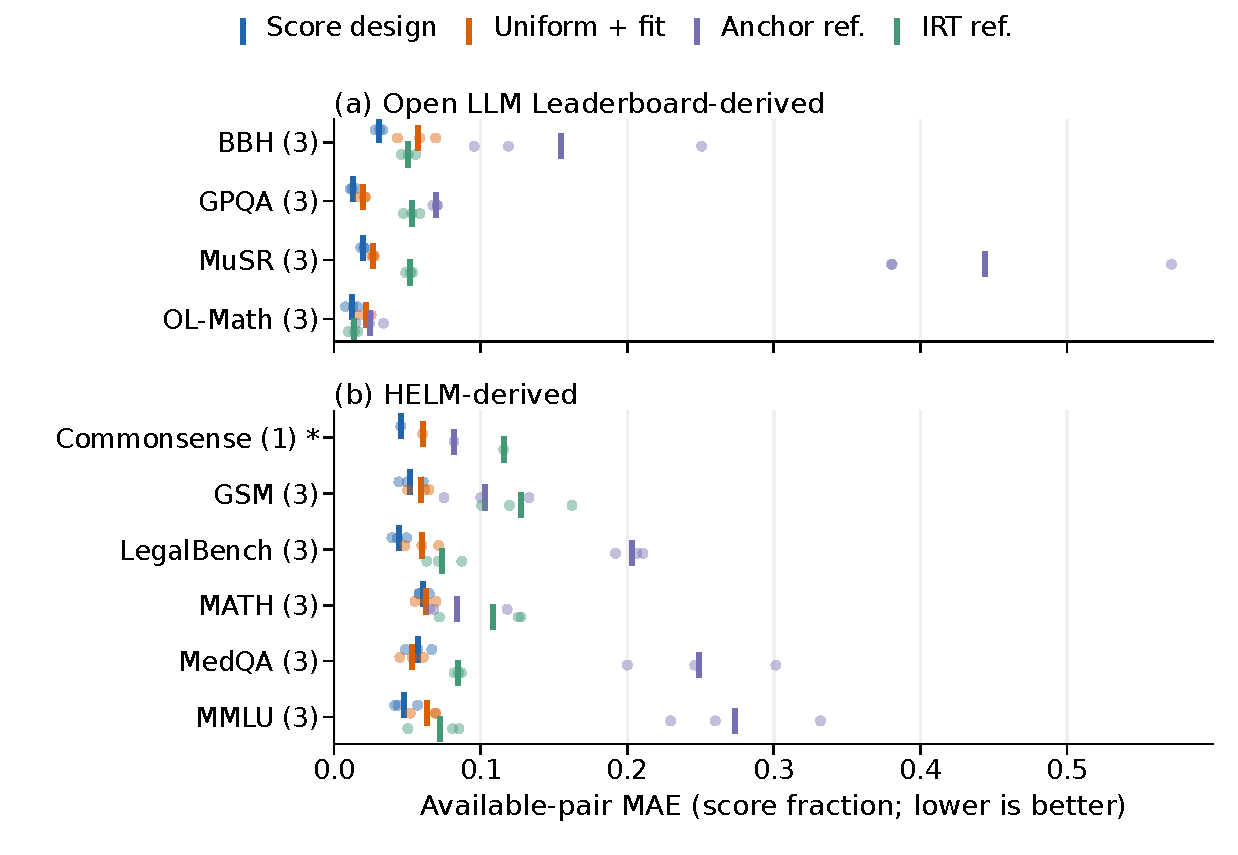
\includegraphics[width=\linewidth]{figures/available_pair_method_comparison.pdf}
\caption{Available-pair MAE, averaged equally over query budgets, separated by data source. Small dots show supported seeds; vertical marks show their descriptive mean. Parentheses give supported seed counts; the asterisk marks missing Commonsense records at seeds 5003 and 9001. All four methods use identical case--seed support. Missing-output penalties are not plotted as measured errors. These conditional results do not restore failed qualification.}
\label{fig:cases}
\end{figure}
% @evidence[[derived_results.json#/case_seed_mae]]

The conditional comparison differs from the reported aggregate ordering because it changes both the available support and the handling of missing records. Neither view should replace the other: the reported aggregate reflects the evaluator's failure policy, while the conditional view describes retained predictions. The latter is compatible with useful prediction accuracy on observed cases and simultaneously insufficient evidence for a qualified overall result. It does not establish that missingness is benign or that the omitted outcomes would follow the same pattern.

\subsection{Item Budget, Reconstruction, and Ranking}
On the stated common-support aggregation, primary MAE is 0.0439, 0.0333, and 0.0278 at the three budgets; fitted uniform-selection MAE is 0.0598, 0.0439, and 0.0328. Figure~\ref{fig:budgets} separates absolute-score prediction from model ranking. Selected-item raw means have much larger MAE (0.1321, 0.1050, and 0.0851), but Spearman correlations of 0.7806, 0.8461, and 0.8819 are close to the primary values of 0.7787, 0.8485, and 0.8858. Reconstruction therefore changes absolute-score error much more than rank correlation in this retained evidence. This is a descriptive matched-order contrast, not an attribution to any one reconstruction component.
% @evidence[[derived_results.json#/budget_mae]]
% @evidence[[derived_results.json#/budget_spearman]]

\begin{figure}[t]
\centering
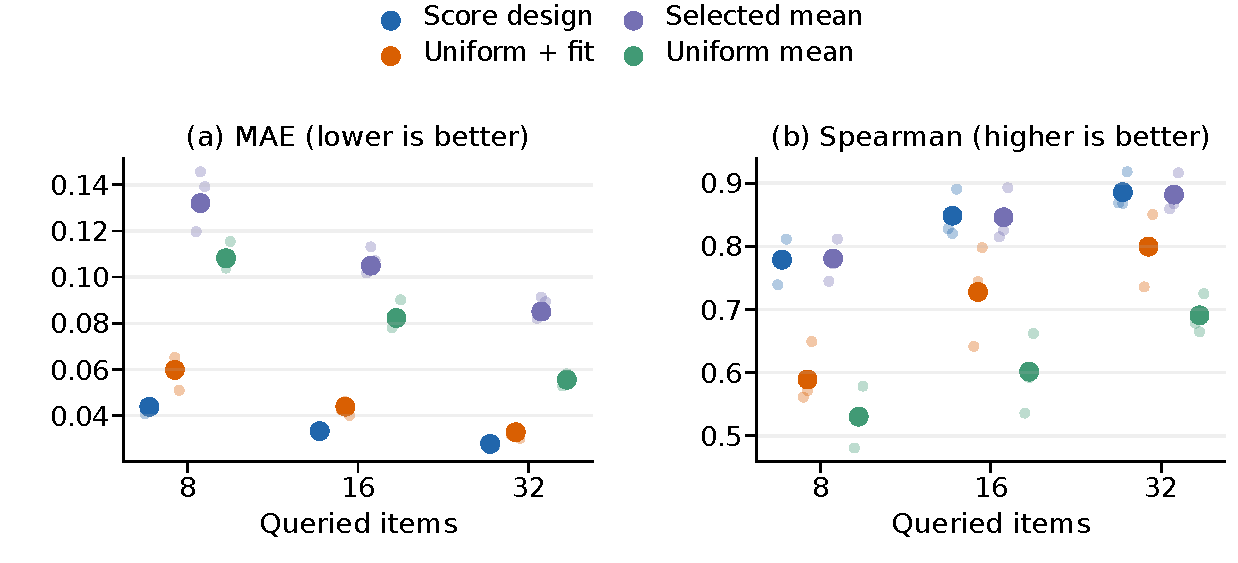
\includegraphics[width=\linewidth]{figures/budget_accuracy_and_ranking.pdf}
\caption{Conditional error and ranking at each budget. Large dots use equal data-source and case weights, with available seeds normalized within each case. Small dots are descriptive seed summaries normalized over cases available for that seed; they are not independent replicates of the pooled estimator. Both panels and all methods use the same available case--seed intersection. No confidence interval or qualified overall comparison is implied.}
\label{fig:budgets}
\end{figure}
% @evidence[[derived_results.json]]

Uniform sample means have lower MAE than selected-item raw means at every displayed budget, whereas fitted selection reverses that ordering on common support. Selection and reconstruction must therefore be assessed jointly. This observation does not identify which selector would be preferable with a fixed independently chosen predictor: the fitted uniform control retunes, and no final fixed-predictor selector-only contrast is available. Similarly, residual-zero and blend-zero settings in source tuning do not constitute independently evaluated final ablations.
% @evidence[[derived_results.json#/budget_mae]]

\section{Discussion and Limitations}
\paragraph{Accuracy is conditional on an evidence mask.}
The main empirical lesson is not simply that one method has a smaller error. A failure policy and an availability-conditioned comparison answer different questions. Worst-case defaults appropriately penalize a non-completing evaluation, but do not reveal how an absent prediction would have scored. Removing those defaults cannot certify completion. Because the missingness mechanism is unknown, we neither impute outcomes nor extrapolate the observed Commonsense split to its missing splits. This distinction remains necessary even when the remaining comparisons look favorable.

\paragraph{What the method comparison identifies.}
The selected-item-mean condition supports a contrast between fitted reconstruction and no reconstruction on the primary prefixes. It does not isolate Rasch smoothing, residual profiles, group balancing, or their interaction. The fitted uniform control changes acquisition and allows downstream retuning, so it compares two configured procedures. Source-validation tuning establishes how settings are selected, not independent evidence that a component improves final performance. Sequentially developed configurations are likewise not controlled component interventions. Missing or unavailable ablations remain missing evidence.

\paragraph{Scope of generalization and uncertainty.}
These are fixed binary benchmarks and metadata-grouped target models, not samples from a defined population of future tasks. Conservative grouping can merge unrelated models or miss undocumented ancestry. The source-trained covariance and profile assumptions can fail under response shifts. Reusing targets across seeds further prevents reading seed dispersion as an independent-sample confidence interval. We retain the evaluator's uninformative paired interval and refrain from replacing it with an unvalidated narrow interval. The checked replay discrepancy only addresses that replay, not arbitrary execution paths or the failed structural conditions.

\paragraph{Scores are not all of evaluation.}
Full-score MAE does not measure item-level probability calibration. A Bernoulli probability score such as the classical Brier criterion \citep{Brier1950} concerns a different prediction object from our reconstructed benchmark average. Likewise, ranking can be approximately preserved even when scores are systematically shifted. No measured deployment cost, CPU speedup over full language-model evaluation, architecture-specific effect, or reliable stopping criterion is established here. The available response matrices avoid new language-model inference, but do not quantify end-to-end operational savings.

\section{Conclusion}
Score-targeted fixed prefixes and source-trained reconstruction provide a concrete approach to few-item benchmark prediction. The retained evaluation supports heterogeneous conditional accuracy comparisons and shows that fitted reconstruction can change score error more than rank ordering on the same selected responses. However, the final assessment completed without qualification: missing primary and reference predictions and failed matched structural checks are essential parts of the result, not peripheral implementation notes.

The reported penalty-scored aggregate and the available-pair reaggregation must therefore remain separate. Neither demonstrates overall superiority, and neither identifies the root cause of the missing outcomes. The available measurements also do not isolate a residual-profile benefit or certify generalization to independent model lineages or new benchmarks. A conclusive evaluation would require complete matched predictions, passing structural checks, and independently assessed component contrasts. Until such evidence exists, the supported conclusion is a bounded account of measured prediction behavior and its unresolved evaluation limits.

\clearpage
\bibliography{references}
\bibliographystyle{paper}

\section*{LLM Usage}
LLM-based agents contributed to method formulation, estimator implementation, literature-query planning, evidence transformation code, and manuscript drafting. The writing step inspected the supplied estimator and evaluator, curated references using exact bibliographic identifiers, and generated descriptive summaries from frozen predictions. It did not generate target answers, fabricate experiments, rerun the final assessment, or use model-generated numerical outputs as independent evidence. Automated checks support artifact consistency; they do not substitute for scientific qualification, independent replication, or human review.

\clearpage
\appendix
\section{Supplementary Information}
\subsection{Inspectable Implementation and Reproducibility}
The accompanying source snapshots are readable evidence, not merely hashes identifying an unavailable implementation. \texttt{source\_evidence/selected\_method.py} contains the evaluated estimator; \texttt{source\_evidence/evaluate\_final.py} contains the evaluator and local references. The entrypoint manifest and method description are preserved alongside them. Table~\ref{tab:locations} gives relevant locations. The estimator is a finite JSON request handler: reset, source transfer, source fitting, prefix observation, and release. It receives binary matrices and opaque source-group labels, not benchmark names or target identities. Predictions are bounded finite scores. Identical observed rows follow the same prediction calculation; reset and release clear learned state.
% @evidence[[source_evidence/program_spec.toml]]
% @evidence[[source_evidence/selected_method.py#L290-L370]]

\begin{table}[h]
\centering\small
\caption{Readable source locations for implementation and protocol claims. Locations refer to the supplied snapshots.}
\label{tab:locations}
\begin{tabular}{ll}
\toprule
Mechanism & File and lines\\
\midrule
Group weighting and score-targeted selection & \texttt{selected\_method.py}, 52--91\\
Ridge and difficulty fitting & \texttt{selected\_method.py}, 94--115\\
Profiles, priors, posterior score & \texttt{selected\_method.py}, 118--191\\
Source-only tuning and final fitting & \texttt{selected\_method.py}, 194--287\\
Model-group split and local references & \texttt{evaluate\_final.py}, 685--771\\
Scored aggregate and paired fallback & \texttt{evaluate\_final.py}, 1005--1076\\
\bottomrule
\end{tabular}
\end{table}

\paragraph{Rebuilding the paper, not rerunning the evaluation.}
The command \texttt{python build\_paper\_artifacts.py} reads only the frozen evidence registry and regenerates \texttt{derived\_results.json}, both quantitative figures, their PDF/PNG exports, and the numerical supplementary tables. Adjacent provenance sidecars identify the inputs. It does not execute the estimator, refit references, query language models, or rerun the sealed assessment. The overview is rendered separately; the rebuild script never overwrites an existing overview. The exact local writing environment and validation commands are documented in \texttt{REPRODUCIBILITY.md}. The original end-to-end environment and a verified full-evaluation runtime are not established by this artifact-only reconstruction; no estimated runtime is presented as a measurement.
% @evidence[[build_paper_artifacts.py]]

\paragraph{Data version and limits of reconstruction.}
The task identifies the pinned binary response-matrix snapshot \texttt{55faff496947789f94e6b5908c77cbc3e84f81ad}. The actual evaluated objects are the staged, filtered matrices described in \texttt{source\_evidence/final\_data\_manifest.json}, not a new download from a moving leaderboard. Its group rule combines recorded base-model relations, aliases/details identities, broad family metadata, and provider fallback. Metadata cannot prove complete lineage separation. Reproducing the evaluation from upstream data requires the staged column alignment and grouping resources as well as the estimator; the frozen predictions alone are sufficient only for the paper's descriptive reaggregation. The original upstream code repository was not accessed during writing under the task's literature restriction.
% @evidence[[source_evidence/final_data_manifest.json]]

\subsection{Extended Estimation Details}
Difficulty initialization uses the group-weighted mean ability minus the logit item mean. Item means are clipped to $[10^{-4},1-10^{-4}]$ for this initialization. Eight Newton updates use group-weighted Bernoulli residuals with difficulty penalty $0.01$ and clip each update to $[-2,2]$. Abilities remain fixed; this is not joint maximum-likelihood Rasch fitting. Profile probabilities are clipped with $\epsilon=10^{-6}$ before applying offsets. Chunked particle summaries avoid retaining the full particle-by-item array during source tuning; a nonzero final blend stores the fitted particle probabilities. A zero blend bypasses that branch at prediction time.
% @evidence[[source_evidence/selected_method.py#L103-L155]]

The source folds rebuild the selected order, Rasch probabilities, profiles, and priors on each fold's training groups. Linear configurations are chosen separately for each budget using equal-group squared error. The profile/blend grid uses MAE averaged over budgets, then rows within groups, then groups. It shares the validation folds with linear tuning, so this score is not an untouched outer-fold performance estimate. If only one source group is supplied, grouped tuning is unavailable and the code uses ridge strength one, shrinkage one, and a zero profile blend. This fallback is a code-defined behavior, not evidence that the final evaluator used a single-group fit.
% @evidence[[source_evidence/selected_method.py#L194-L287]]

Equation~\ref{eq:profile} explicitly separates known and predicted items. In the batch path, the expected unqueried total is computed as each particle's full expected total minus its queried expected total. The single-row path sums over an explicit unqueried mask. Both implement the same algebra. This source inspection supports an implementation description, not an empirical guarantee that every execution path passed the evaluator's controls. The final diagnostic failures remain in force.

\subsection{Local Reference Implementations}
The anchor reference centers each item's source response vector, normalizes its length, and applies $k$-means with $k=b$, one initialization, and at most 30 iterations. Representatives are distinct nearest response vectors. Every item is reassigned to its nearest representative and representative weights are the fractions assigned. Target score prediction is the weighted average of queried responses. This reference need not match the preprocessing, optimization, or benchmark regime of published Anchor Points.
% @evidence[[source_evidence/evaluate_final.py#L711-L729]]

The IRT reference models logits as $\theta_i\exp(\eta_j)-d_j$. Its objective is summed Bernoulli negative log likelihood plus penalties $0.5\|\theta\|^2+0.05\|\eta\|^2+0.005\|d\|^2$. L-BFGS-B uses bounded parameters and at most 40 iterations. Item order is the decreasing fitted information $a_j^2 p_j(1-p_j)$ at zero ability, where $a_j=\exp(\eta_j)$ \citep[Chap.~6]{Baker2001}. Target abilities use up to 30 regularized Newton updates on queried responses; the reference score averages fitted response probabilities over the entire item universe. Finite-objective checks do not prove solver optimality. No exact reproduction of a published IRT benchmark-compression package is claimed.
% @evidence[[source_evidence/evaluate_final.py#L732-L771]]

\subsection{Available-Pair Numerical Results}
Table~\ref{tab:cases_si} retains exact case-level descriptive means to more precision than the main text. All methods within a row use the same supported seeds and give equal weight to each budget and target within a seed. The table is not an extrapolation to absent records. In particular, the Commonsense row is a single split, and cannot quantify its between-seed stability.
\begin{table}[h]
\centering
\caption{Conditional MAE on common available support. $n$ counts supported seeds.}
\label{tab:cases_si}
\begin{tabular}{lrrrrr}
\toprule
Case & $n$ & Score design & Uniform + fit & Anchor & IRT\\
\midrule
% BEGIN GENERATED case_mae
% @evidence[[paper_data.json#/final_evaluation/evaluation_evidence/episodes]]
BBH & 3 & 0.0308 & 0.0570 & 0.1551 & 0.0507 \\
GPQA & 3 & 0.0128 & 0.0197 & 0.0694 & 0.0530 \\
MuSR & 3 & 0.0198 & 0.0266 & 0.4441 & 0.0515 \\
OL-Math & 3 & 0.0123 & 0.0221 & 0.0242 & 0.0132 \\
Commonsense & 1 & 0.0455 & 0.0605 & 0.0818 & 0.1157 \\
GSM & 3 & 0.0517 & 0.0590 & 0.1027 & 0.1275 \\
LegalBench & 3 & 0.0440 & 0.0599 & 0.2031 & 0.0738 \\
MATH & 3 & 0.0603 & 0.0624 & 0.0838 & 0.1083 \\
MedQA & 3 & 0.0574 & 0.0530 & 0.2492 & 0.0845 \\
MMLU & 3 & 0.0474 & 0.0634 & 0.2738 & 0.0721 \\
% END GENERATED case_mae
\bottomrule
\end{tabular}
\end{table}
% @evidence[[derived_results.json#/case_mae]]

\begin{table}[h]
\centering
\caption{Conditional budget summaries. Cases receive equal weight within source domain, domains equal weight, and available seeds equal weight within case. Raw selected means and reconstructed scores use the same primary prefixes.}
\label{tab:budget_si}
\begin{tabular}{rlrr}
\toprule
Items & Method & MAE & Spearman\\
\midrule
% BEGIN GENERATED budget_metrics
% @evidence[[paper_data.json#/final_evaluation/evaluation_evidence/episodes]]
8 & Score design & 0.0439 & 0.7787 \\
8 & Uniform + fit & 0.0598 & 0.5892 \\
8 & Selected mean & 0.1321 & 0.7806 \\
8 & Uniform mean & 0.1082 & 0.5303 \\
16 & Score design & 0.0333 & 0.8485 \\
16 & Uniform + fit & 0.0439 & 0.7278 \\
16 & Selected mean & 0.1050 & 0.8461 \\
16 & Uniform mean & 0.0823 & 0.6015 \\
32 & Score design & 0.0278 & 0.8858 \\
32 & Uniform + fit & 0.0328 & 0.7995 \\
32 & Selected mean & 0.0851 & 0.8819 \\
32 & Uniform mean & 0.0556 & 0.6908 \\
% END GENERATED budget_metrics
\bottomrule
\end{tabular}
\end{table}
% @evidence[[derived_results.json#/budget_mae]]
% @evidence[[derived_results.json#/budget_spearman]]

\subsection{Seed-Level Records and Exhaustive Numerical Ledger}
Table~\ref{tab:seed_si} gives the recorded primary metrics for every case--seed pair, averaged equally over budgets. The target count and number of recorded target-group labels vary with the split. A missing primary record stays missing in this table rather than inheriting its evaluator penalty. This table retains the affected rows explicitly, while the main aggregate table preserves the separately scored defaults.
% @evidence[[paper_data.json#/final_evaluation/evaluation_evidence/episodes]]

\begin{table}[p]
\centering\small
\setlength{\tabcolsep}{3pt}
\caption{All primary case--seed records. $T$ counts targets and $H$ their recorded groups. Errors and correlations average the three budgets. Missing outputs are not measured errors; available rows do not repair failed overall qualification.}
\label{tab:seed_si}
\begin{tabular}{lrrrrrrr}
\toprule
Case & Seed & $T$ & $H$ & MAE & RMSE & Spearman & Kendall\\
\midrule
% BEGIN GENERATED primary_seed_metrics
% @evidence[[paper_data.json#/final_evaluation/evaluation_evidence/episodes]]
BBH & 5003 & 54 & 10 & 0.0281 & 0.0349 & 0.8109 & 0.6488 \\
BBH & 7001 & 65 & 10 & 0.0311 & 0.0395 & 0.8239 & 0.6577 \\
BBH & 9001 & 243 & 10 & 0.0331 & 0.0432 & 0.9250 & 0.7658 \\
GPQA & 5003 & 54 & 10 & 0.0110 & 0.0149 & 0.6439 & 0.4973 \\
GPQA & 7001 & 64 & 10 & 0.0123 & 0.0155 & 0.7122 & 0.5326 \\
GPQA & 9001 & 243 & 10 & 0.0152 & 0.0203 & 0.8333 & 0.6467 \\
MuSR & 5003 & 54 & 10 & 0.0182 & 0.0234 & 0.7836 & 0.6100 \\
MuSR & 7001 & 65 & 10 & 0.0209 & 0.0272 & 0.6419 & 0.4624 \\
MuSR & 9001 & 244 & 10 & 0.0203 & 0.0255 & 0.7730 & 0.5790 \\
OL-Math & 5003 & 54 & 10 & 0.0078 & 0.0122 & 0.7274 & 0.6130 \\
OL-Math & 7001 & 65 & 10 & 0.0129 & 0.0208 & 0.7905 & 0.6874 \\
OL-Math & 9001 & 244 & 10 & 0.0161 & 0.0243 & 0.9037 & 0.7588 \\
Commonsense & 5003 & 14 & 5 & \multicolumn{4}{c}{Missing; not a measured loss} \\
Commonsense & 7001 & 20 & 5 & 0.0455 & 0.0737 & 0.8867 & 0.7742 \\
Commonsense & 9001 & 37 & 5 & \multicolumn{4}{c}{Missing; not a measured loss} \\
GSM & 5003 & 14 & 5 & 0.0500 & 0.0611 & 0.9288 & 0.7763 \\
GSM & 7001 & 20 & 5 & 0.0442 & 0.0552 & 0.9424 & 0.8403 \\
GSM & 9001 & 37 & 5 & 0.0608 & 0.0731 & 0.9336 & 0.8052 \\
LegalBench & 5003 & 14 & 5 & 0.0394 & 0.0524 & 0.7651 & 0.6237 \\
LegalBench & 7001 & 20 & 5 & 0.0431 & 0.0518 & 0.8429 & 0.6652 \\
LegalBench & 9001 & 35 & 5 & 0.0496 & 0.0625 & 0.7919 & 0.6375 \\
MATH & 5003 & 14 & 5 & 0.0650 & 0.0762 & 0.9782 & 0.9098 \\
MATH & 7001 & 20 & 5 & 0.0580 & 0.0683 & 0.9414 & 0.8517 \\
MATH & 9001 & 37 & 5 & 0.0580 & 0.0827 & 0.9340 & 0.8079 \\
MedQA & 5003 & 14 & 5 & 0.0666 & 0.0798 & 0.8548 & 0.6726 \\
MedQA & 7001 & 20 & 5 & 0.0571 & 0.0752 & 0.8665 & 0.7133 \\
MedQA & 9001 & 37 & 5 & 0.0485 & 0.0623 & 0.9262 & 0.7864 \\
MMLU & 5003 & 14 & 5 & 0.0570 & 0.0775 & 0.9560 & 0.8618 \\
MMLU & 7001 & 20 & 5 & 0.0437 & 0.0619 & 0.9129 & 0.7678 \\
MMLU & 9001 & 37 & 5 & 0.0413 & 0.0577 & 0.8682 & 0.7126 \\
% END GENERATED primary_seed_metrics
\bottomrule
\end{tabular}
\end{table}

An exhaustive machine-readable table, \texttt{complete\_metrics.csv}, additionally retains every recorded condition and reference, separated by case, seed, and budget. It includes primary, both fitted/raw-mean controls, matched constant/copied/permuted observations, replay where recorded, and anchor/IRT/uniform/source-mean references. Missing prediction metrics are blank, not penalty values; availability and structural-failure fields remain separate. As in the evaluator, a constant truth or prediction vector receives rank correlation zero by convention. Scores for a condition with a failed structural check describe its recorded output only, not validated performance. The table and its provenance sidecar are generated by the same transformation script as the figures.
% @evidence[[complete_metrics.csv]]
% @evidence[[source_evidence/evaluate_final.py#L874-L882]]

For completeness, the remaining reported diagnostic MAEs are 0.2220 for constant observations, 0.1545 for copied observations, 0.1005 for permuted observations, and 0.0281 for replay. These evaluator summaries have their original weighting and scope; they are not new controlled accuracy estimates. In particular, replay covers the checked repeated case rather than the full benchmark collection, and matched corrupted observations are not ordinary target responses.
% @evidence[[paper_data.json#/final_evaluation/metrics/constant_mae]]
% @evidence[[paper_data.json#/final_evaluation/metrics/copy_mae]]
% @evidence[[paper_data.json#/final_evaluation/metrics/permuted_mae]]
% @evidence[[paper_data.json#/final_evaluation/metrics/reset_mae]]

\subsection{Availability Masks and Statistical Interpretation}
There are 30 planned case--seed pairs, of which 28 enter the common-support comparisons. For the budget plots, each available pair supplies all three budgets and all four displayed methods. The per-case normalization deliberately preserves the intended relative mass of the two data sources. It does not make the missing splits exchangeable with the retained split. A globally normalized available-pair average would be a different statistic; neither is an estimate of the complete evaluation without a missingness assumption.
% @evidence[[derived_results.json#/common_support]]

The seed dots in the budget figure separately renormalize the original case weights over cases available for each seed. Consequently their average need not equal the large pooled dot, whose normalization is within each case. They convey descriptive variation under overlapping model-group partitions and should not be used as independent replicates for a significance test. No new bootstrap or inferential procedure is introduced by the paper's plotting code. All qualification facts remain those of the frozen evaluator.

Structural checks use matched constant, copied, and permuted observations to test dependence on legal observations, together with reset replay. Their aggregate failure summary is not an ordinary proportion of independent failed target models. Likewise, the missing-evaluation fraction counts scheduled evaluation units, including conditions and replay, not case--seed pairs. The two missing primary pairs and their baseline omissions are therefore reported explicitly rather than inferred from that fraction.
% @evidence[[source_evidence/evaluate_final.py#L1070-L1095]]

\end{document}
